\chapter{Mathematics Primer}

\begin{quote}The power of equations lies in the philosophically difficult
correspondence between mathematics, a collective creation of human minds, and an
external physical reality.  Equations model deep patterns in the outside world.
By learning to value equations, and to read the stories they tell we can uncover
vital features of the world around us.  In principle, there might be other ways
to achieve the same result.  Many people prefer words to symbols; language, too,
gives us power over our surroundings.  But the verdict of science and technology
is that words are too imprecise, and too limited, to provide an effective route
to deeper aspects of reality.  They are too coloured by human-level assumptions.
Words alone can't provide the essential insights.

Equations can.

-Ian Stewart, {\it In Pursuit of the Unknown, 2012}
\end{quote}


\section{Introduction}

Mathematics is a language not expressed in words but in symbols.  You might
start to wonder if mathematicians are an alien race with their own language or
at the very least an international cabal trying to promote a Greek as a global
language.  We use math because it is the most efficient and effective way to
portray quantitative information and ideas.  One of the beauties of mathematics
is that it is universal, by this I mean that it doesn't matter what language you
natively speak and what words you attribute to the symbols it holds the same
intrinsic meaning.  Because of its power, geophysics is awash with mathematics
and you will need a reasonable level of competence to fully grasp the concepts
in this course.

The purpose of this maths primer is to cover a great deal of the background
mathmematics that you will need to understand this course to the fullest extent
possible.  Read over them once early in the course and then refer back to
specific sections as they arise throughout the course. 

If you suffer from math-phobia---as a great number of people do---the largest
obstacles to learning math are mental blocks that are self-created.  Many
spectacular scientists are math-phobic, but have learned to resist the self
imposed limits of understanding when the need arises.  If there are math
concepts that you do not understand ask for help from myself, the demonstrators,
your peers.  There is also the Maths Learning Centre, a campus resource that
anyone can utilize.


\subsection{HELP!!! Maths Learning Centre}

Level 3 East, Hub Central, North Terrace Campus

The Maths Learning Centre (MLC) helps all students learn and use the maths they
need at uni (including statistics). They specialise in helping people improve
their confidence and skills for learning maths. The MLC offers seminars,
workshops, online and print resources and also a drop-in service.

{\bf MLC Drop-In room -- Level 3 Hub Central} \\
Staffed 10am to 4pm, Monday to Friday during teaching weeks, SWOT and exams. 
No appointment needed, come as often as you want, stay as long as you need.
Talk to a staff member about anything mathematical relating to your course.

{\bf MLC Resources for this course}
Resources to help you succeed with the maths relating to this course may be
found on the MLC website at
\url{adelaide.edu.au/mathslearning/resources/}.

For further information: \\
phone: \href{tel:+61-8-8313-5862}{8313 5862} \\
e-mail: \url{mailto:mathslearning@adelaide.edu.au} \\
web: \url{adelaide.edu.au/mathslearning/}.

\subsection{Common Symbols}

\begin{table}[hbt]
    \centering
    \caption{Greek alphabet.\vspace{2pt}}
    \label{tab:mathsym}
    \begin{tabular}{@{}clclcl@{}}
        \toprule
        Letter &
        Name &
        Letter &
        Name &
        Letter &
        Name \\
        \midrule
        $\mathrm{A}$, $\alpha$     & alpha &
        $\mathrm{I}$, $\iota$      & iota  &
        $\mathrm{P}$, $\rho$ or $\varrho$ & rho \\

        $\mathrm{B}$, $\beta$      & beta  &
        $\mathrm{K}$, $\kappa$     & kappa &
        $\Sigma$, $\sigma$     & sigma \\

        $\Gamma$, $\gamma$      & gamma &
        $\Lambda$, $\lambda$    & lambda &
        $\mathrm{T}$, $\tau$       & tau \\

        $\Delta$, $\delta$      & delta &
        $\mathrm{M}$, $\mu$        & mu &
        $\Upsilon$, $\upsilon$  & upsilon \\

        $\mathrm{E}$, $\epsilon$ or $\varepsilon$ & epsilon &
        $\mathrm{N}$, $\nu$        & nu &
        $\Phi$, $\phi$ or $\varphi$ & phi \\

        $\mathrm{Z}$, $\zeta$      & zeta  &
        $\Xi$, $\xi$            & xi &
        $\mathrm{X}$, $\chi$       & chi \\

        $\mathrm{H}$, $\eta$       & eta   &
        $\mathrm{O}$, $\mathrm{o}$    & omicron &
        $\Psi$, $\psi$          & psi \\

        $\Theta$, $\theta$ or $\vartheta$ & theta &
        $\Pi$, $\pi$            & pi &
        $\Omega$, $\omega$      & omega \\
        \bottomrule
    \end{tabular}
\end{table}

\begin{table}[hbt]
    \centering
    \caption{Other symbols.\vspace{2pt}}
    \label{tab:symbols}
    \begin{tabular}{@{}ccl@{}}
        \toprule
        \textbf{Symbol} & \textbf{Name} & \textbf{Use} \\
        \midrule
        $x$ & {} & scalar \\
        $\vb{x}$ & {} & vector\\
        $\mat{x}$ & {} & matrix \\
        $\sim$ & {} & approximately \\
        $\approx$ & {} & approximately equal to \\
        $\sum$ & sum operator & summation \\
        $\prod$ & product operator & product analogy to summation \\
        $\infty$ & {} & infinity \\
        $\to$ & goes to & used for limits \\
        $\partial$ & partial & partial derivative \\
        $d$ & infintesimal & derivatives/integration \\
        $\nabla$ & nabla or del & vector differential operator \\
        $\int$ & anti-derivative/integral & integration \\
        $\hat{}$ & hat & denotes unit vector \\
        $\dagger$ & dagger & denotes complex conjugate \\
        \bottomrule
    \end{tabular}
\end{table}

\section{Big and Small Numbers}

Sometimes the numbers we discuss get very big or very small.  As you can see
from the table below, writing out the full number can get very cumbersome---not
to mention hard to read.  Imagine haveing to count the number of zeros every
time just to see how big a number is.  Never fear, there is a shorthand.  Either
we can divide the number by a conveniently large or small number and use the SI
shorthand, or we can write the number as a power of ten (Table~\ref{tab:pot}).
\begin{table}[hbt]
    \centering
    \caption{Powers of ten.}
    \label{tab:pot}
    \begin{tabular}{@{}lcclc@{}}
        \toprule
        \textbf{name} & \textbf{SI prefix} & \textbf{SI symbol} & $10^x$ & \textbf{number} \\
        \midrule
        septillion & yotta & Y & $10^{24}$ & 1 000 000 000 000 000 000 000 000 \\
        sextillion & zetta & Z & $10^{21}$ & 1 000 000 000 000 000 000 000 \\
        quintillion & exa & E & $10^{18}$ & 1 000 000 000 000 000 000 \\
        quadrillion & peta & P & $10^{15}$ & 1 000 000 000 000 000 \\
        trillion & tera & T & $10^{12}$ & 1 000 000 000 000 \\
        billion & giga & G & $10^9$ & 1 000 000 000 \\
        million & mega & M & $10^6$ & 1 000 000 \\
        thousand & kilo & k & $10^3$ & 1 000 \\
        hundred & hecto & h & $10^2$ & 100 \\
        ten & deca & da & $10^1$ & 10 \\
        one & {} & {} & $10^0$ & 1 \\
        tenth & deci & d & $10^{-1}$ & 0.1 \\
        hundreth & centi & c & $10^{-2}$ & 0.01 \\
        thousandth & milli & m & $10^{-3}$ & 0.001 \\
        millionth & micro & $\mu$ & $10^{-6}$ & 0.000 001 \\
        billionth & nano & n & $10^{-9}$ & 0.000 000 001 \\
        trillionth & pico & p & $10^{-12}$ & 0.000 000 000 001 \\
        quadrillionth & femto & f & $10^{-15}$ & 0.000 000 000 000 001 \\
        quintillionth & atto & a & $10^{-18}$ & 0.000 000 000 000 000 001 \\
        sextillionth & zepto & z & $10^{-21}$ & 0.000 000 000 000 000 000 001 \\
        septillionth & yocto & y & $10^{-24}$ & 0.000 000 000 000 000 000 000 001 \\
        \bottomrule
    \end{tabular}
\end{table}

To write a number, $x$, as a power of ten we simply count the digits to the left
(if $x > 1$) or right (if $x < 1$) of the decimal to the most significant digit.
If $n$ is our number of digits and $x > 1$, the order is $n-1$ and $x < 1$ than
one, the order is $n$.  Examples:
\begin{align}
    12300 &= 1.23 \times 10^4 , \\
    0.0321 &= 3.21 \times 10^{-2} . \\
\end{align}

Numbers written in this manner, $a \times 10^b$, are often said to be in {\it
scientific notation}.  Beyond making large and small numbers eaiser to read, we
can use this scientific notation to simplify multiplication and division.  In
fact, you'll be encouraged to do this a number of times throughout the course as
you perform back-of-the-envelope calculations.  To multiply two numbers
expressed in scientific notation, we multiply each mantissa ($a$) and add the
exponents ($b$).  Example:
\begin{align*}
    6 \times 10^3 * 2 \times 10^{-4} = (6 \cdot 2) \times 10^{(3 + (-4))} \\
    &= 12 \times 10^{-1} \\
    &= 1.2 \times 10^{0}.
\end{align*}
As above, sometimes we need to adjust power of 10 following the operation.

Your calculator and computers often write numbers this way both because
calculations are faster and it saves memory.  However, when a calculator or
computer write scientific notation, they also tend to shorten it by $a \times
10^b$ to $a\,\mathrm{e}\,b$ or $a\,\mathrm{E}\,b$, where $\mathrm{e}$ and $\mathrm{E}$
substitute for $\times 10$. 


\section{Accuracy versus Precision}

The goal of observation is to be {\it precise} and {\it accurate}.  However, we
must be careful because they do not mean the same thing.  Precision
results from the sensistivity of an instrument or other measurement and
represents how repeatable an observation may be made.  Accuracy is being close
to the truth, although, this may be closeness in an average sense rather than as
the result of any singe observation.

It is possible to be precise and not accurate (Fig.~\ref{fig:avp}) when an
instrument is miscalibrated, your location is incorrect, or there is some other
systematic bias to the data.  In general, it is better to sacrifice precision
for accuracy if the choice must be made.
\begin{figure}
    \centering
    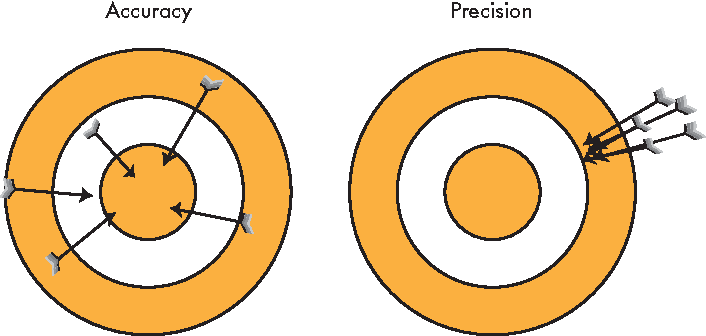
\includegraphics[]{math_primer/figures/accuracy_vs_precision.eps}
    \caption{The difference between accuracy and precision.  On the left, the
    arrows are accurate, but not precise.  Those on the right are precise, but
    not accurate.}
    \label{fig:avp}
\end{figure}


\section{Significant Digits}

Even though your computation yields a long list of digits doesn't mean we need
all of them.  For example, $5/6 = 0.8333333...$; however, we only have one
significant digit in 5 and 6, hence our answer should be written as one
significant digit as 0.8.  To determine the number of significant digits count
the number of digits between preceeding and trailing zeros.

Why do we care about significant digits?  Every instrument we use perform a
measurement has a scale.  The smallest change in a quantity the instrument can
report is the precision (e.g. the shortest distance between ticks on a ruler).
Any numbers that are reported below that number are an estimate or purely
ficticious.  We can reasonably keep one estimated digit, but all others should
be dropped.  Note: trailing zeros can be significant if our measuring device
reports a trailing zero.

As we perform mathematical operations, we should keep in mind the number of
significant digits for each of our quantities and report our answer with the
same number of significant digits as our least precise quantity.  The
significant digits of our physical constants should also be taken into an
account (although most have greater precision than our measurements).  Although,
a constant such as $2$ in our equation (e.g., kinetic energy $= \frac{1}{2} m
v^2$) can be assumed to have infinite precision (so don't round to one digit
based on it alone).

There are a couple rules for rounding (we'll use the simplist one).  Take the
last significant digit.  If it is $\geq$5, round the preceeding digit up,
otherwise truncate after the most significant digit.  An example is provided
below (Table~\ref{tab:sigdig}).
\begin{table}[hbt]
    \centering
    \caption{Significant digits for 7288.1345 to varying precision.}
    \label{tab:sigdig}
    \begin{tabular}{cl}
        \toprule
        \textbf{Significant digits} & \textbf{Rounded result} \\
        \midrule
        8 & 7288.1345 \\
        7 & 7288.135 \\
        6 & 7288.13 \\
        5 & 7277.1 \\
        4 & 7277 \\
        3 & 7280 \\
        2 & 7300 \\
        1 & 7000 \\
        \bottomrule
    \end{tabular}
\end{table}

\section{Basic Math Concepts}

\subsection{What is a function?}

In the previous section, we described a field as a function.  But what exactly is it and how do we use it in geophysics?  A function performs and operation or set of operations on an input.  Hence, for the specified domain (set of points), $x$, the function, $f$, transforms $x$ into a new domain, $y$,
\[
    x \mapsto f(x) = y.
\]

To specify the domain of $x$, we will use $[\,]$ to specify a closed domain, which includes the end-points, and $(\,)$ to specify a open domain, which excludes the end-points.  For example, suppose we use the function $f(x) = r^{-2}$ to describe some physical relationship where the domain over which it is valid lies from $0$ to $R$ but not including $R$.  In this case, we would say that $r \in [0,R)$, where $\in$ means ``is an element of.''  You might be wondering why we make a distinction between a domain that includes an end-point or not.  Some physical processes change their functional form (shape) at a boundary, yield a value different than the function would predict, or the result is undefined at a boundary.  For instance this occurs for an electric field perpendicular to a geologic boundary where the resistivity changes.

Most physical processes result in only one solution and are said to be single-valued, for each input their is exactly one output.  However, there are times the mathematical functions we use to describe a process are multi-valued, multiple possible output to a single input.  For example, the function $f(x) = x^{1/2}$ is a multi-valued function.  Because both positive and negative numbers yield a positive value when squared, the square-root is ambiguous and could yield either a positive or negative value.  Generally when we need a multi-valued function to describe a process we will add a restriction that makes it single valued.  For instance, for $f(x) = x^{1/2}$ we limit the solution to a positive result.

The above example also brings forth an important point.  The inverse to a function performs an operation, such that the identity set is returned.  As a simple example,
\[
    f[f^{-1}(x)] = x.
\]
In geophysics, we wish to understand the distribution of a particular property (or set of properties) given the response of physical effect. For gravity, it is rather simple to write down a function for gravity with a known distribution of masses.  We call this the \emph{forward problem} and is rather simple to write down as a single-valued mathematical function.  However, we measure the gravitational force or acceleration due to an unknown distribution of masses.  This formulation is the \emph{inverse problem}.  For many inverse problems, it is far more difficult to write down a single-valued function because there are often multiple valid solutions, e.g., mass distributions that can lead to the same measured data.  This nonuniqueness is especially true when the data have some level of uncertainty, which is always the case.  In this text, we begin by focusing on forward problems. In later parts of the sequence we return to inverse problems and develop more sophisticated tools to handle their non-uniqueness and instability.

\subsection{Continuity and Differentiability Definitions}

For a function to be continuous, it must not have any steps, holes (a single undefined point in an otherwise smooth function), or divergent limits.  If you were asked to draw a function and were forced to pick up the pencil, the function would be discontinuous.  A function can also be continuous but not differentiable if it has sharp corners (cusps), which commonly occur at physical boundaries leading to phenomena like refraction. We will forgo a more rigorous definition since this explanation is sufficient for our needs.

In physics, many functions become discontinuous at boundaries, but are continuous in the regions in between.  In this case, we call our functions piece-wise continuous.
\begin{center}
    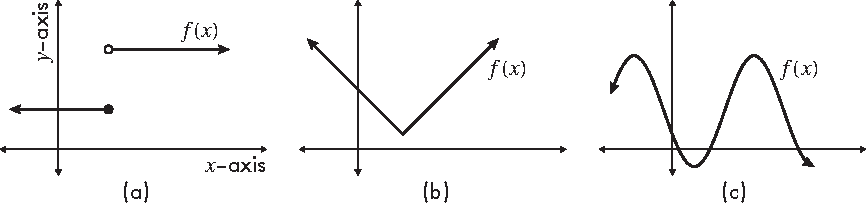
\includegraphics[]{introduction/figures/contdiff.pdf}
    \captionof{figure}{Examples of different types of functions. (a) Discontinuous or
    piecewise continuous. (b) Continuous but not differentiable. (c) Continuous
    and differentiable.}
\end{center}

A function is said to be differentiable if the derivative exists everywhere throughout its defined domain.  But again, there are locations, typically boundaries, where the derivative does not exist or only as a limit from one side.  For a function to be differentiable, it must be continuous and smoothly varying (i.e., no radical changes in slope).  A function can be continuous but not differentiable.  For example $f(x) = \abs{x}$ is continuous everywhere, but not at $x = 0$.

\clearpage
\nocite{Schey1997}
